% Appendix B

\chapter{Simulated Annealing} % Main appendix title

This appendix justify the name of the quantum approach we use in the present work -- \textit{Quantum Anneling} (QA) -- to solve \textit{Quadratic Unconstrained Binary Optimization} (QUBO) problems. In next sections, we show that the expressions we get in the classical approach known as \textit{Simulated Annealing} (SA), have the same functional form as the ones we get with QA. To do that we are gonna develop the solution for a stochastic problem. For a better understanding about stochastic problems see \cite{Schneider2006StochasticOptimization}. 
\label{AppendixB} % For referencing this appendix elsewhere, use \ref{AppendixB}
\section{Master Equation}
\subsection{Discrete Processes}
Suppose we have a space of states $\Gamma = \{\uparrow \uparrow,\downarrow \uparrow,\uparrow \downarrow,\downarrow \downarrow \} \equiv \{1, 2, 3, 4 \}$ and a discrete stochastic process so that $\{X_{t}, t= 0,1,2,...\} \rightarrow \{1,4,2,3,1,..\}$. Furthermore, assume that the actual setting of our system only depends on the previous one, i.e., the probability of being in state \textit{j} at time \textit{t+1}, $X_{t+1}= j$, given that the current state is \textit{i}, $X_{t} = i$, does not depend on previous configurations. Mathematically,
\begin{equation}
\label{eq: MarkovChain}
    P\left(X_{t+1} = j | X_{t} = i\right) = P\left(X_{t+1}=j | X_{t} = i, X_{t-1} =i_{t-1},...,X_{0} = i_{0}\right)
\end{equation}
The equation \ref{eq: MarkovChain} is known as \textbf{Markov Chain} condition and the conditional probabilities are named \textit{transition probabilities}.\\
The normalization condition for probabilities is also fulfilled, i.e, starting from a state  \textit{i} any state \textit{j} -- where \textit{j} can be also the current state -- has a transition probability such that
\begin{equation}
    \sum_{j}P\left(X_{t+1} = j | X_{t} = i\right) = 1, \;\; \forall i
\end{equation}
Graphically, this means that the current state of our systems has to be in a given state of $\Gamma$ at any time.
\begin{figure}[H]
    \centering
    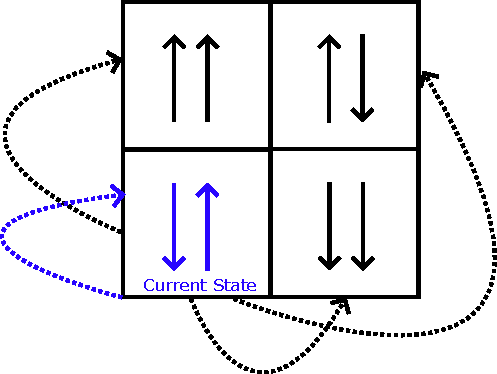
\includegraphics[scale=0.65]{Figures/SA_StateJump.pdf}
    \caption{Stochastic Process for a configuration space $\Gamma$ of four states.}
    \label{fig:SimulatedAnneling_StatesJump}
\end{figure}
\begin{theorem}[Total Probability]
Given an event A in a discrete set of events $\{B_{i}\}$. The probability of ocurrence of event A is given by,
\begin{equation}
    P\left(A\right) = \sum_{i}P\left(A|B_{i}\right)P\left(B_{i}\right)
\end{equation}
where $P\left(A|B_{i}\right)$ is the probability of occurrence of event A given that event $B_{i}$ has already happened. 
\end{theorem}
Renaming variables,
\begin{align}
    \label{eq:Renaming1}
    \Pi_{i}(t) := P\left(X_{t} = i\right) \\
    \label{eq:Renaming2}
    p_{i \leftarrow j} := P\left(X_{t+1} = i | X_{t}=j\right)
\end{align}
From equations \ref{eq:Renaming1} and \ref{eq:Renaming2}, we can write,
\begin{align}
        \Pi_{i}(t+1) = p_{i \leftarrow i}\Pi_{i}(t) + \sum_{j \neq i} p_{i \leftarrow j}\Pi_{j}(t) \\ 
        p_{i \leftarrow i} = 1 - \sum_{j\neq i}p_{j \leftarrow i}
\end{align}
combining last two equations,
\begin{align}
    \Pi_{i}(t+1) = \left[1 - \sum_{j\neq i}p_{j \leftarrow i}\right]\Pi_{i}(t) + \sum_{j\neq i}p_{i \leftarrow j}\Pi_{j}(t)\\
    \Pi_{i}(t+1) - \Pi_{i}(t) = -\Pi_{i}(t) \sum_{j \neq i}p_{i \leftarrow j} + \sum_{j \neq i} p_{i \leftarrow j}\Pi_{j}(t) \\
    \label{eq: MasterEquationDiscrete}
    d\Pi_{i}(t) := \Pi_{i}(t+1) - \Pi_{i}(t) =  -\Pi_{i}(t) \sum_{j \neq i}p_{i \leftarrow j} + \sum_{j \neq i} p_{i \leftarrow j}\Pi_{j}(t)
\end{align}
we get the master equation of a Markov stochastic discrete process.
\subsection{Continuous Processes}
In case we deal with a continuous process, we need to work with transitions rates defined by,
\begin{equation}
    \mathcal{L}_{i \leftarrow j} = 
    \begin{cases}
    \mathcal{L}_{i \leftarrow j} \;\; i\neq j\\
    -\sum_{k\neq i}\mathcal{L}_{k \leftarrow i} \;\; i = j
    \end{cases}
\end{equation}
so that the master equation can be written as,
\begin{equation}
\label{eq: MasterEquationContinuous}
    \frac{d\Pi_{i}(t)}{dt} = \sum_{j}\mathcal{L}_{i \leftarrow j} \Pi_{j}(t)
\end{equation}
If we know $\Pi_{i}(t_{0})$ we can know the probability at each state. Assume our system has reached the stationary state, i.e.,  $\frac{d\Pi_{i}}{dt} = 0$, which implies,
\begin{equation}
\label{eq: StationaryCondition}
    \Pi_{i}^{eq} \sum_{j\neq i} \mathcal{L}_{j \leftarrow i} = \sum_{j \neq i}\mathcal{L}_{i \leftarrow j}\Pi_{j}^{eq} 
\end{equation}
A sufficient but not necessary condition to fulfill \ref{eq: StationaryCondition} is,
\begin{equation}
    \Pi_{i}^{eq}\mathcal{L}_{j \leftarrow i} = \mathcal{L}_{i \leftarrow j}\Pi_{j}^{eq} 
\end{equation}
which is knonw as \textbf{detailed balanced condition}.\\
The evolution of our system is determined knowing an initial state and the transition rate expression. Metropolis et. al. have chosen Bolztmann distribution, so,
\begin{equation}
    \Pi_{i}^{eq} = \frac{1}{Z}exp\left(- \frac{\mathcal{H}_{i}}{k_{B}T}\right), \;\;\; Z = \sum_{i}exp\left(-\frac{\mathcal{H}_{i}}{k_{B}T}\right)
\end{equation}
which implies,
\begin{equation}
    \frac{\mathcal{L}_{j \leftarrow i}}{\mathcal{L}_{i \leftarrow j}} = exp\left(\frac{\mathcal{H}_{i} - \mathcal{H}_{j}}{k_{B}T}\right)
\end{equation}
The last expression does not define uni-vocally the transition rate so we need a criteria for that. There are two common criteria:
\begin{itemize}
    \item\textbf{ Metropolis Criteria:} $\mathcal{L}_{j \leftarrow i} = min \left[1,exp\left(\frac{\mathcal{H}_{i}-\mathcal{H}_{j}}{k_{B}T}\right)\right]$. This condition guarantee a transition into states with lower energy without forbidding a transition to high energy states, where this transition rate is given by the energy difference. 
    \item \textbf{Thermal Bath criteria:} $\mathcal{L}_{i \leftarrow j} = \frac{\Pi_{j}^{eq}}{\Pi_{i}^{eq} + \Pi_{j}^{eq}} = \left[1 + exp\left(\frac{\mathcal{H}_{j}- \mathcal{H}_{i}}{k_{B}T}\right)^{-1}\right]$ 
\end{itemize}
 The transition rates do not guarantee the optimal value of our objective function. Including a time dependence of temperature guarantee reaching the optimal value in $t \rightarrow \infty$. 
\subsection{Annealing Schedules}
The annealing approach consider a temperature starting from a high value so it decreases gradually with time. The dependence of temperature with respect time t is named annealing schedule. There are many annealing schedules but the most common are \footnote{From now on, $k_{B} = 1$.},
\begin{itemize}
    \item \textbf{Geman-Geman:} $T(t) = \frac{a}{b + \log{t}}$
    \item \textbf{Lineal Cooling:} $T(t) = a - bT$ where $a = T_{0}$ -- initial temperature -- and $b \in (0.01,0.2)$.
    \item \textbf{Exponential Cooling:} $T(t) = ab^{t}$ where $a = T_{0}$ -- initial temperature -- and $b \in (0.8,0.999)$.
\end{itemize}
Choosing the annealing shcedule is one of the trickest part of annealing problems. If we chose an shchedule that guarantee a miniaml value of our cost function then the required time tends towards $\infty$. In case we choose a quick schedule for out problem, the effectivity of our algorithm to find the minimal value is compromised.
\section{Objective Function}
\begin{equation}
    \label{eq: SA_ObjectiveFunction}
    \mathcal{H} = -\sum_{i,j} \mathcal{J}_{ij}s_{i}s_{j} - \underbrace{h\sum_{i}s_{i}}_{Zeeman\;Term}
\end{equation}
where $\mathcal{J}_{ij}$ measure the interaction between spins $\{s_{i},s_{j}\}$ \textit{ij} and \textit{h} is the magnetic field.